\section{Testing Strategy: Force Requirement Validation \& Three-Tier Testing}

Testing in Part 2 is governed by two things: a fixed structure for what gets tested and at what level, and a mandatory reasoning step that has to happen before a failing test is touched.

The structure is a three-tier testing strategy, where each tier targets a different class of problem and none substitutes for another. The first tier is backend integration testing with pytest, required for every new endpoint, using the Flask test client against an in-memory database rather than the production one. The second tier is a frontend smoke test using React Testing Library, required for every new component; the requirement is deliberately minimal --- asserting only that the component renders without crashing when given its expected props --- kept intentionally cheap so that its cost is never a reason to skip it. The third tier is browser-based end-to-end verification, required for any feature that touches the user interface and exempted only for backend-only changes: the backend and frontend are started, the feature is exercised in the browser exactly as a user would, and the result --- correct routing, UI state, error messages, and API responses --- is confirmed visually, with a screenshot taken for each verified behavior and attached to the implementation's walkthrough document (\Cref{fig:e2e-permission-collections,fig:e2e-permission-invite}).

\begin{figure}[H]
    \centering
    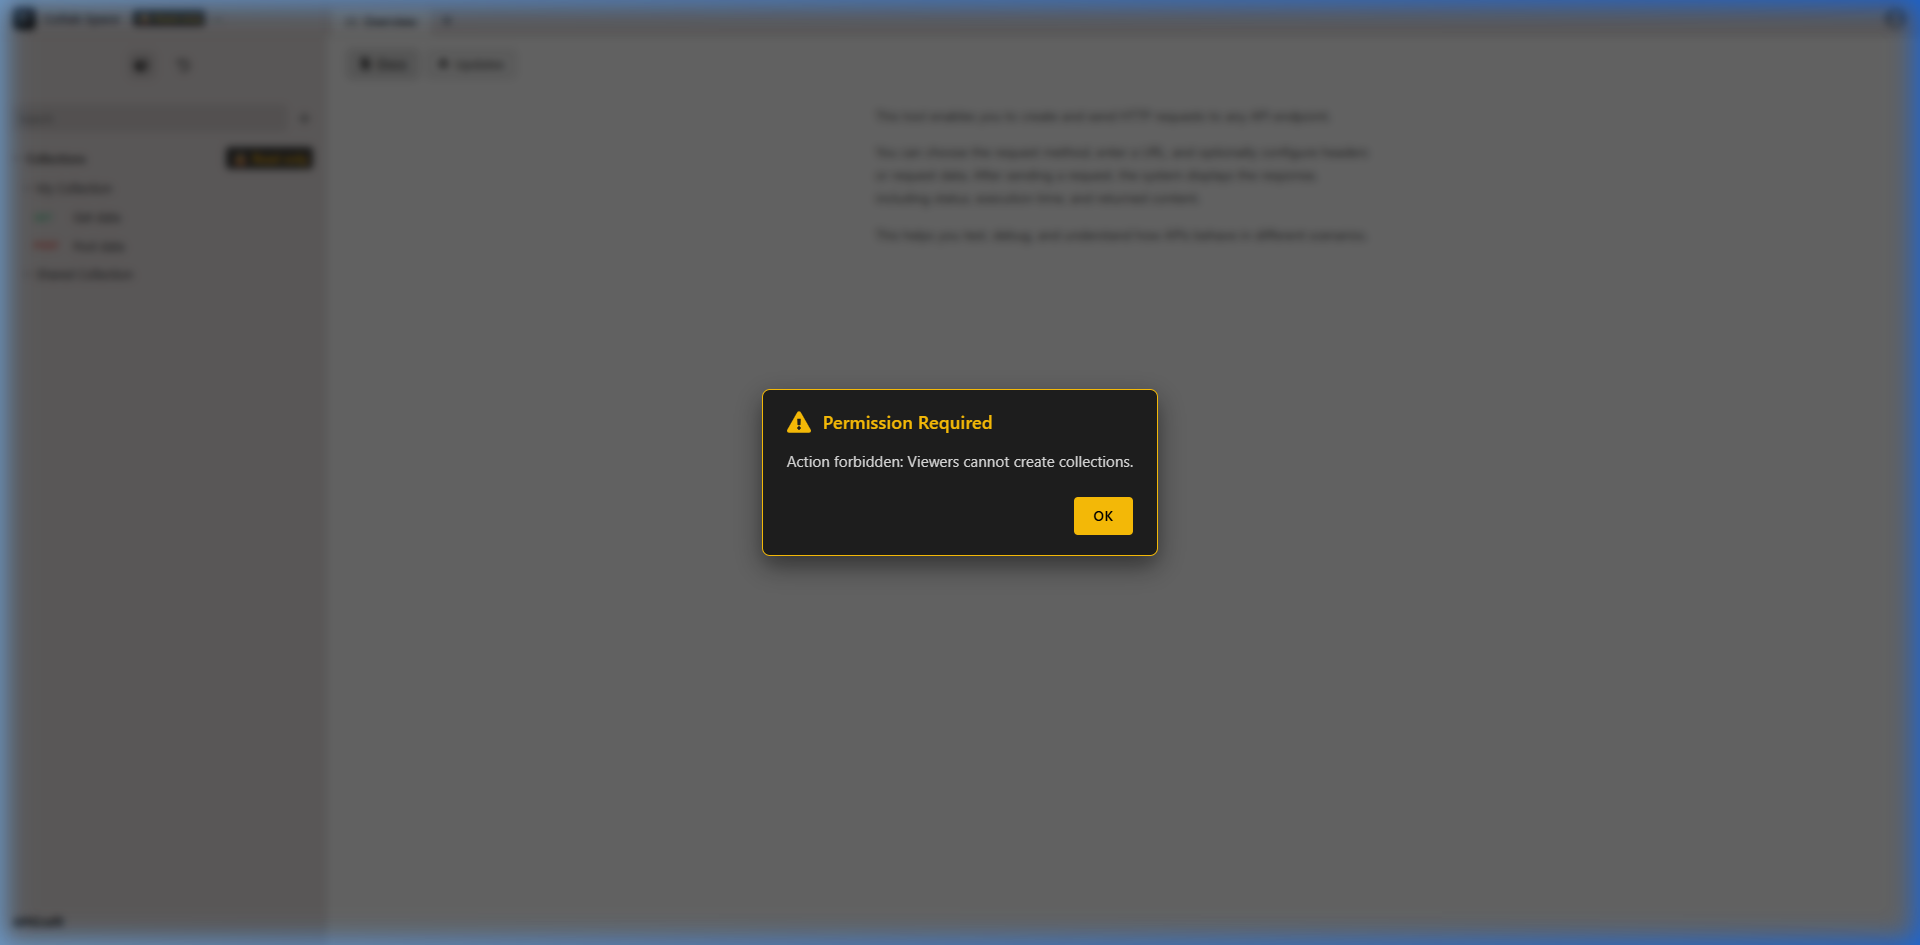
\includegraphics[width=0.85\linewidth]{Bilder/Part2-StructuredApproach/e2e_permission_collections.png}
    \caption{Browser-based verification of a permission error: a viewer-role user is blocked from creating a collection.}
    \label{fig:e2e-permission-collections}
\end{figure}

\begin{figure}[H]
    \centering
    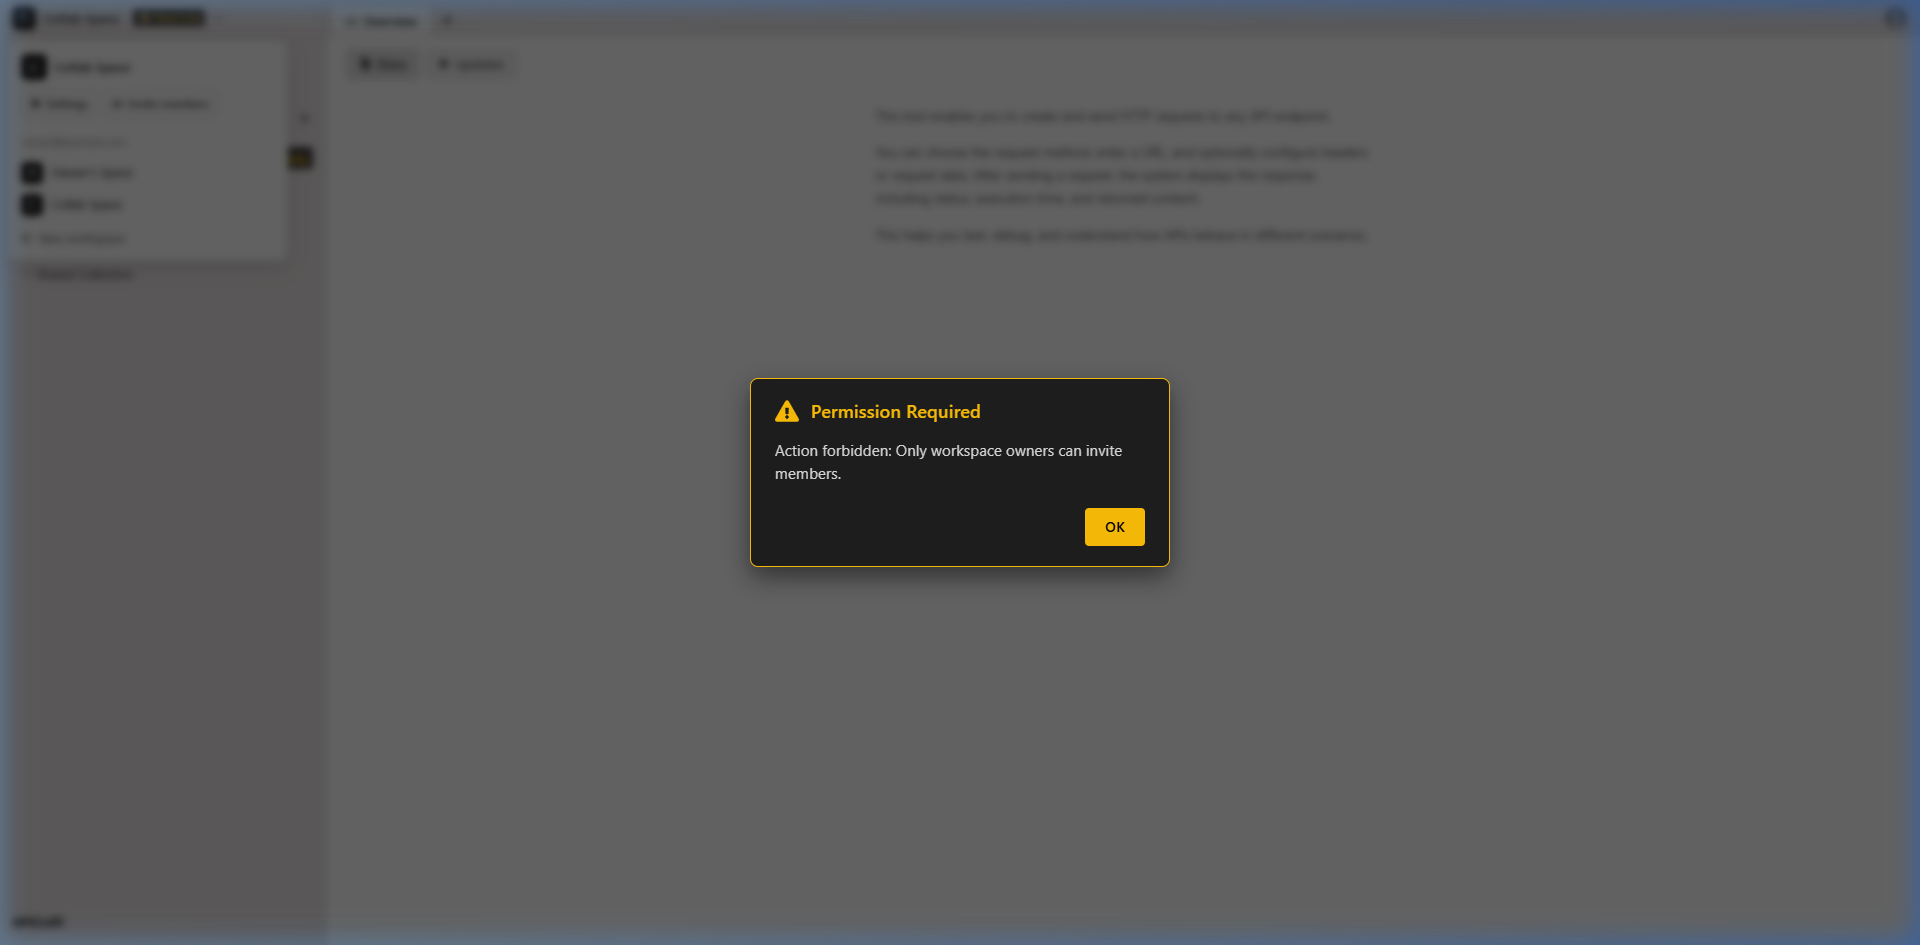
\includegraphics[width=0.85\linewidth]{Bilder/Part2-StructuredApproach/e2e_permission_invite.png}
    \caption{Browser-based verification of a permission error: a non-owner is blocked from inviting workspace members.}
    \label{fig:e2e-permission-invite}
\end{figure}

Layered on top of this structure is a rule about where tests are allowed to come from. Tests must be derived from the requirements stated in the feature's plan, not from whatever the implementation happens to do --- for every requirement listed, at least one test has to verify it directly, and each requirement's coverage has to include a normal case, an error or unauthorized case, and any boundary condition the feature explicitly calls for. A feature cannot be marked complete if any requirement lacks a corresponding test, even if every test that does exist is passing. This addresses directly what had been observed as a recurring risk: that an agent, left to its own judgment, could satisfy the letter of "the tests pass" while never actually testing whether the feature does what it was asked to do.

The second half of the testing strategy governs what happens when a test fails. Before making any change, the agent is required to first read the test to understand what it asserts, then read the implementation to understand what it currently does, and only then decide --- and state explicitly, in writing, before touching anything --- whether the fault lies with the implementation, with the test's own expectation, or, following the same reasoning already established through Part 1's collection-seeding case, with a requirement that was never clearly defined in the first place. Only once that determination has been made and recorded is either the implementation or the test allowed to be changed, and never both at once as an unexamined guess. This turns what had been, in Part 1, a lesson learned from a single incident into a mandatory procedure applied to every failing test regardless of how minor it seems.

